    Figure \ref{pipeline} shows the experiment data pipeline. Data is imported from the NXT switchboard corpus \cite{calhoun2010nxt} into a graph database \cite{Webber:2012:PIN:2384716.2384777}.
   Figure \ref{datastructure} shows the data structure as it is represented inside the graph database. For each conversation, the conversation entities (words, dialog acts and turns) are represented as edges between time points, which are represented as vertices. The structure leads to a direct computation of the summary features using the graph query language.
\begin{figure}[ht!]
 \centering
 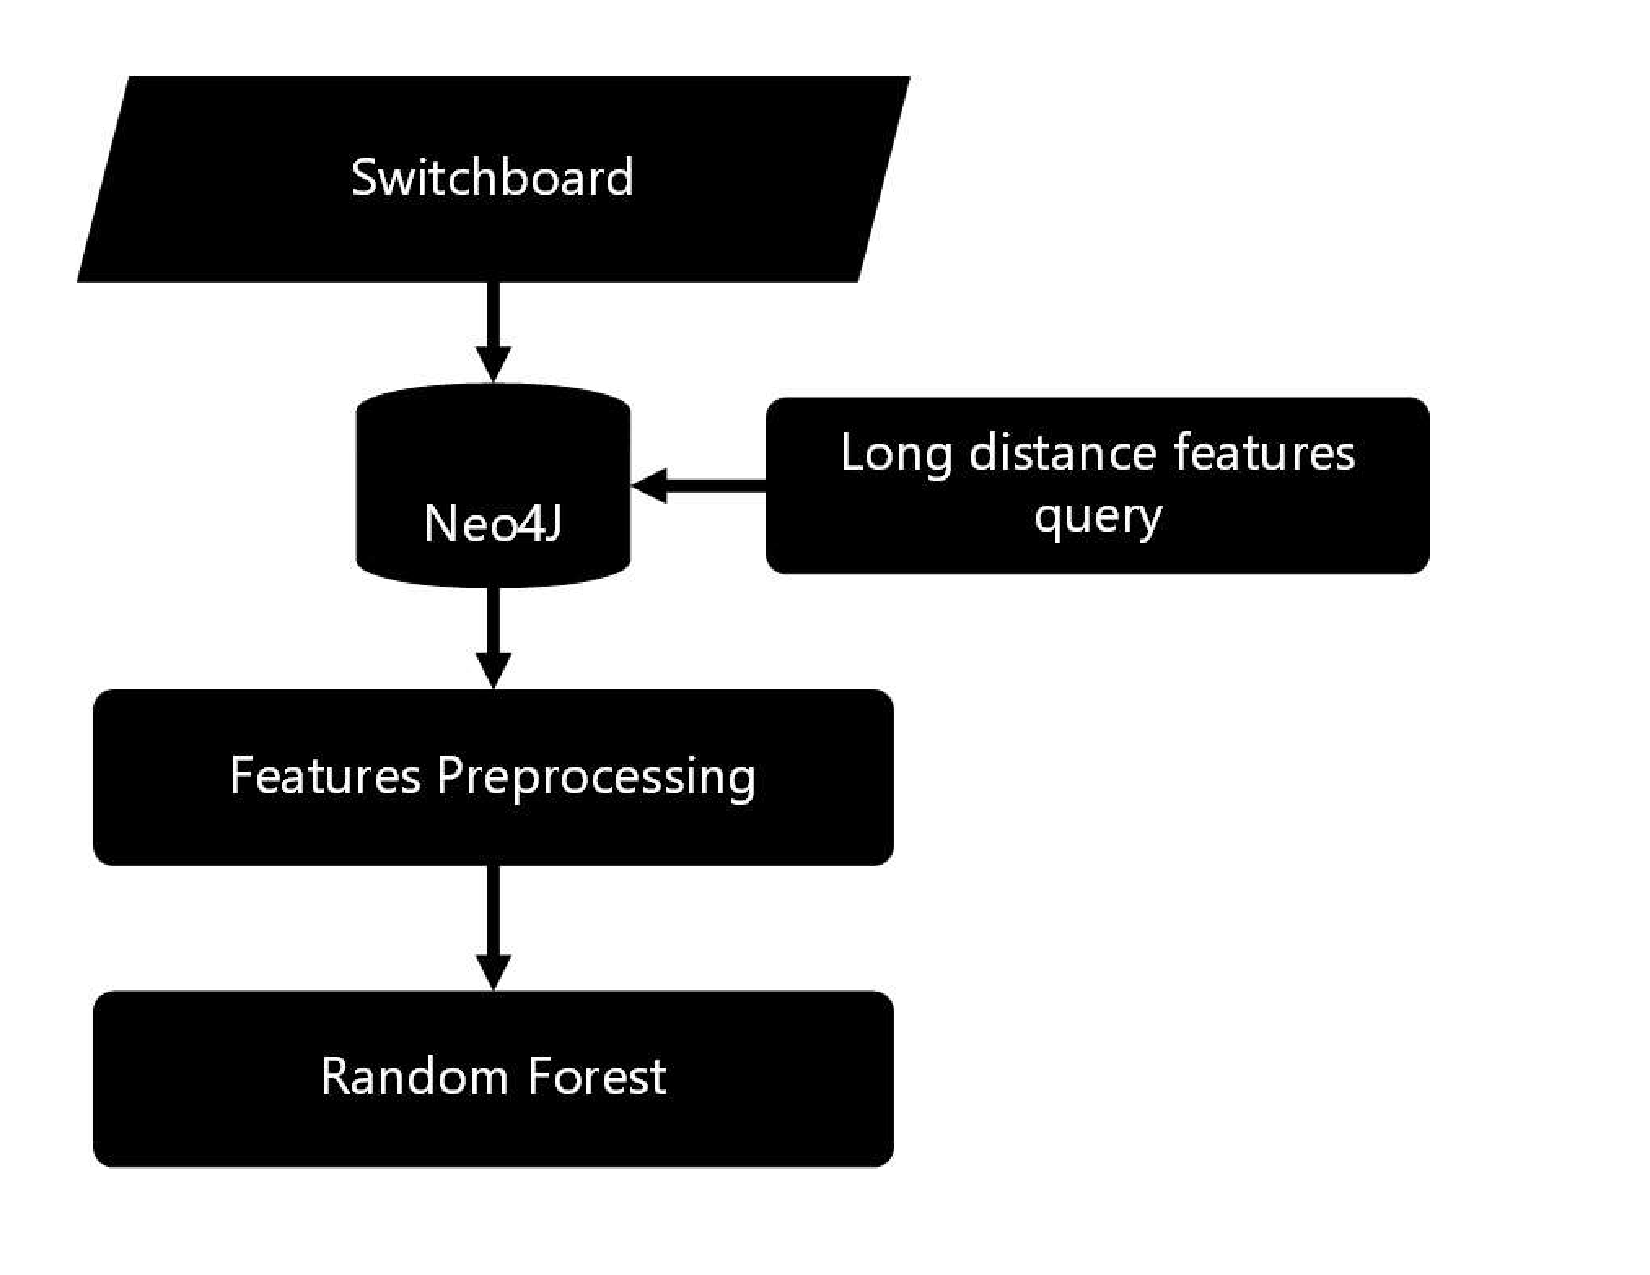
\includegraphics[width=10cm,keepaspectratio]{pipeline1.pdf}
 \caption{Experiment data pipeline
 \label{pipeline}}
 \end{figure}



\begin{figure}[ht!]
\centering
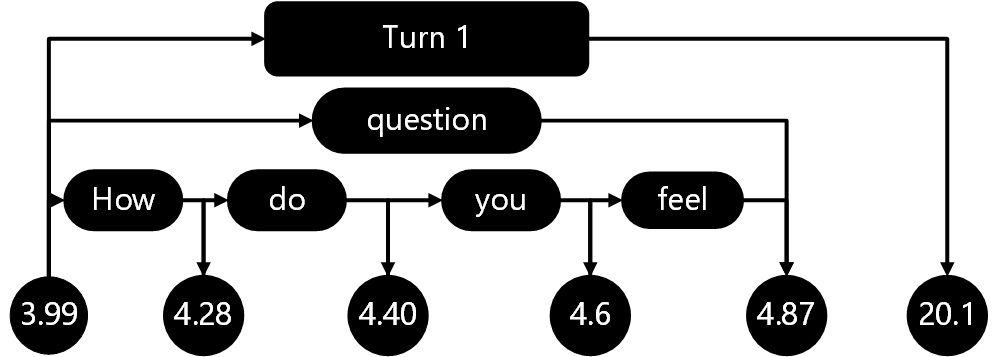
\includegraphics[width=10cm,keepaspectratio]{graph5.jpg}
\caption{Conversation graph data model \label{datastructure}}
\end{figure}

   After computing the summary features, we perform the following data transformation:
    \begin{itemize}[leftmargin=1em]
    \item We exclude 11 dialogue acts that were coded in Switchboard as ``other.''
    \item Since we believe that it takes a certain amount of time to build a stable conversational image, in evaluating our model, we removed all turns that occurred in the first part of each conversation. For this paper, we used an estimate of 120 seconds. This reduced the number of dialog acts from 50,633 to 37,508.
    \item To reduce data sparsity, we grouped switchboard dialog acts into dialog act classes. This reduced the number of dialog acts from 148 to 9 dialog act classes. See Table 1 for examples of the mapping.
    \item We added a binary $y_{i+1}$ feature to each dialog act. As explained in Section 3, the variable is 1 if there is a turn change from dialogue act $d_i$ to $d_{i+1}$.

    \end{itemize}
    \begin{table}
     \begin{center}
    \begin{tabular}{ |p{2cm}||p{3cm} | }
    \hline
Switchboard dialog acts &  Dialog act classes  \\
    \hline
sd,h,bf      & statement   \\
sv,ad,sv@    & statement - opinion  \\
aa,aa\^r     & agree accept \\
\%.\%-,\%@   & abandon      \\
b,bh         & backchannel  \\
qy,qo,qh     & question     \\
no,ny,ng,arp & answer       \\
+            & +            \\
o@,+@        & NA           \\
  \hline
\end{tabular}
\end{center}\vspace{-0.5em}
\caption{Mapping from dialog act to dialog act class}
\label{tab:mapping}
\end{table}


\subsection{Classification Models}

    To test the contribution of the summary features, we used a binary classifier with
    $y_i$ as the outcome variable. We trained four models, which used the following sets of features:

    \begin{description}
        \item[baseline 1:] Predict turn transition based only on the current dialog act label.
        \item[baseline 2:] Predict turn transition based on the labels of the current and previous dialog acts.
        \item[summary model:] Predict turn transition using just the summary features.
        \item[full model:] Predict turn transition using the summary features and the current and previous dialog acts.
    \end{description}


We used random forests to build the binary classifiers $(N=200)$ \cite{Breiman01randomforests}. Random forests build an ensemble of decision trees during training, and during testing, each decision tree votes on the outcome.  Like decision trees, they can account for interactions between variables, such as making greater use of the summary features when the current speech act is not a question.  Random forests though are not as sensitive to overfitting and data fragmentation.

To find the optimal hyper parameters, we ran a grid search over the \textit{max\_features} and \textit{max\_depth} hyper parameters for each model. The hyper parameters search was done over $\{sqrt, log2, 10\}$ for \textit{max\_features} and $\{5, 7, 9\}$ for \textit{max\_depth}. When training the model, we used the optimal hyper parameters for each feature set.

   We performed 10 fold-labeled cross validations.  We made sure that each conversation was entirely in a single fold. This way, each dialogue was entirely used for training or testing, but never for both at the same time.
